\documentclass[tikz, border=10pt]{standalone}

\usetikzlibrary{arrows}

\begin{document}
	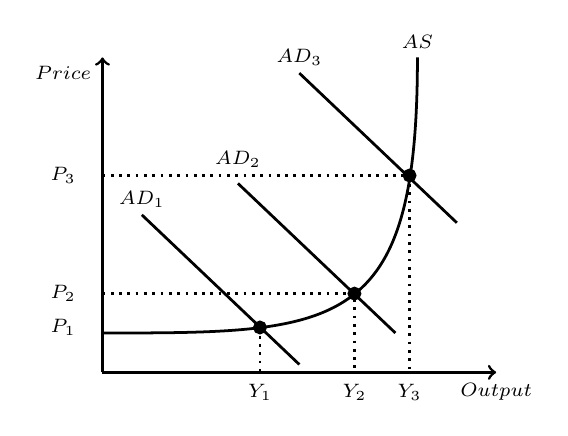
\begin{tikzpicture}[line width=1pt]
	% Нарисовать горизонтальную и вертикальную линии
	\draw[->] (0, 0) -- (5, 0);
	\draw[->,color=black] (0, 0) -- (0, 4);

	% Нарисовать AS
	\draw (0, 0.5) .. controls (3, 0.5) and (4, 0.5) .. (4,4);
	
	% AD#
	\draw (0.5, 2) -- (2.5, 0.1);
	\draw (1.72, 2.4) -- (3.72, 0.5);
	\draw (2.5, 3.8) -- (4.5, 1.9);
	
	% Точки
	\draw[fill=black] (2, 0.57) circle (2pt);
	\draw[fill=black] (3.2, 1) circle (2pt);
	\draw[fill=black] (3.9, 2.5) circle (2pt);
	
	\draw[dotted] (2, 0.57) -- (2, 0);
	\draw[dotted] (0, 1) -- (3.2, 1) -- (3.2, 0);
	\draw[dotted] (0, 2.5) -- (3.9, 2.5) -- (3.9, 0);

	\begin{scriptsize}
		\draw (-0.5, 3.8) node {$Price$};
		\draw (5, -0.25) node {$Output$};
		
		\draw (-0.5, 0.57) node {$P_{1}$};
		\draw (-0.5, 1) node {$P_{2}$};
		\draw (-0.5, 2.5) node {$P_{3}$};
		
		\draw (2, -0.25) node {$Y_{1}$};
		\draw (3.2, -0.25) node {$Y_{2}$};
		\draw (3.9, -0.25) node {$Y_{3}$};
		
		\draw (0.5, 2.2) node {$AD_{1}$};
		\draw (1.72, 2.7) node {$AD_{2}$};
		\draw (2.5, 4) node {$AD_{3}$};
		
		\draw (4, 4.2) node {$AS$};
	\end{scriptsize}
	\end{tikzpicture}
\end{document}




